\begin{savequote}[10cm] % this sets the width of the quote
\sffamily
 In 1980 there was no Internet or cell phone network, most people did not travel by air, most of the advanced medical technologies in common use today did not yet exist, and only a minority attended college. In the areas of communication, transportation, health, and education, the changes have been profound. These changes have also had a powerful impact on the structure of employment: when output per head increases by 35 to 50 percent in thirty years, that means that a very large fraction— between a quarter and a third— of what is produced today, and therefore between a quarter and a third of occupations and jobs, did not exist thirty years ago.\cite{RefWorks:447}
\qauthor{Thomas Piketty}
\end{savequote}

\chapter{The Australian Internet Economy}

\subsection{Main Message}
The economy is dependent on technology to function efficiently. ICT amplifies the speed at which money can circulate and, combined with social interactions, can build a new economy that is networked and amplified by social interactions. ICT has the ability to eliminate the differences between urban and non--urban environments if non--urban areas are able to access equivalent levels of service in networking and communications technology as urban Australians. Remote and regional Australians have been historically disadvantaged by not having good access to ICT resources and have therefore been relegated to interacting with the economy through last generation technology. The NBN promises, for the first time, to give uniform access Australia wide to ICT and hence access to the same level of access to the economy in very remote and remote areas that urban and some inner regional centres have enjoyed.

Australians have had economic systems as long as there have been human inhabitants on the continent. Reciprocity, a system of trade that predates money has been in effect in Australia since human habitation. This system was made more efficient by the movement of people and their goods from areas with few resources to areas with more resources and back again. With the introduction of non-Indigenous economy to Australia, technology has been used to connect the Australian economy to the international economy. Money is virtual and lends itself to being transmitted, and stored electronically. Using technology to handle money magnifies its effect on the lives of the people who use it by increasing its circulation and therefore its benefit through the economy. Regional and remote economies have lower quality communications networks than their urban counterparts and are disadvantaged by a heavy reliance on cash and the expense of working through human agents who collect fees, interest and charges to provide this cash. Australia is at the forefront of a worldwide conversion of its economy from a cash based to cashless economy. Regional and remote areas of Australia are being targeted for cashless economy even as the infrastructure necessary to facilitate such an economy lags behind the urban Australian economy due to the high cost of processing transactions in non--urban centres.

\subsection{Size of the Internet economy in Australia}
When considering the economy of the entire World, the term Gross World Product is sometimes used which is the combined totals of all Gross Domestic Products (GDP)s. Since the World is a single economic entity in itself so the World can be said to have a GDP as well.  In 2017, the global economy (GWP/GDP) was estimated to be over AUD 110 Trillion (USD~80.6 Trillion) in 2018.  Australia's GDP in 2017 was estimated to be AUD~1.8Trillion  (USD~1.3 Trillion) making Australia's economy the thirteenth largest economy in the World\cite{RefWorks:448}. Every month the payments platforms of Australian banks and credit card processors move AUD~1 Trillion (USD~730 Billion) around the economy\cite[p29]{CAFS2018}. The speed at which these funds moves, its velocity, is greatly facilitated by the internet and amplifies the utility of this cash transfer. This economy is bigger than that of countries such as Spain, South Korea, Mexico, Indonesia and Saudi Arabia and constitutes over 1.5\% of the global economy.\cite{RefWorks:293}
The entire World economy is affected by the internet but the internet-only economy or `digital economy' has around 3.2 billion people and is worth around AUD~4 trillion (USD~2.9 Trillion) in 2016. 
\begin{quotation}
\ldots[T]his is about 30\% of the S\&P 500, six times the U.S.' annual trade deficit or more than the GDP of the United Kingdom.  What's more is that this entire value has been generated in the past 20 years since the launch of the Internet.
It has consolidated value at record speed. The path to half a trillion in 20 years or less is an extremely impressive feat --- American free enterprise at its finest.  [\ldots]  But equally interesting is how rapidly the path from start-up to value consolidation has been.  The Digital Economy may still be in its adolescence but 9 companies currently generate 90\% of its revenue and profits --- Apple, Google, Facebook and Amazon (popularly known as the ``four horsemen''), Microsoft, and the four Chinese digital giants.  Everyone else you've heard about or think you've heard about (for example, Yahoo, Twitter, eBay, Snapchat, Pinterest, Uber or others) is barely over 10\% of this economy.\cite{RefWorks:295}
\end{quotation}


The digital economy as defined by the Australian Government is `the global network of economic and social activities that are enabled by information and communications technologies, such as the internet, mobile and sensor networks.'\cite[p9]{RefWorks:274} 

The accounting firm, Deloitte has studied the digital economy in both 2011 and 2015 and concluded that it is larger in size than the agriculture, transport or retail industries. They estimate that the digital economy `contributed AUD~79 billion (or 5.1\% of GDP in 2013--14) and had grown 50\% in size' since they last measured it in 2011. Deloitte concluded that the digital economy could expand to be worth AUD~139 billion by 2020(7.3\%) of GDP)\cite[p1]{RefWorks:274} The digital economy is enabled, improved and enhanced by ICT and current innovations such as cloud computing, machine learning and big data analytics may enhance the contribution of ICT to the economy such that further growth beyond 7.3\% can be expected. The report calls out the contribution of ICT to business transformation and the fact that ICT is benefiting government services which traditionally are not counted towards GDP. The report nominates the benefit to the government of ICT services as \$7 billion/year. For comparison,this is about the same as the amount the Australian Federal Government spends individually on, Public Schools or Roads or Health Services\cite{RefWorks:276}. ICT benefits education, transportation and health so each of these would presumably require a higher budget were it not for the efficiencies brought by ICT.

The Deloitte report also notes that `the internet and digital technologies could have contributed between \$45 to \$92 billion to the Australian economy in 2013, approximately 2.9\% to 5.9\% of Australia's annual GDP.'\cite[p14]{RefWorks:275} and that they made a difference of \$1,959 per capita, raising average GDP per capita from around \$64,000 to approximately \$66,000 per capita.[p15]


This economy does not encompass all economic activity in Australia. The contribution of unwaged and volunteer work to the economy is especially large {\color{red} how large?}

The `shadow' economy, where earnings are paid in cash but not declared to government institutions such as the taxation office, will not be shown in formal GDP statistics but nevertheless contribute to the economy. The Australian government estimates that the size of the `shadow' economy is no more than 2.5\% of GDP which, for 2017 when Australia's GDP was AUD1,679billion\cite{ABS1345}  would equate to around AUD42billion/year. International agencies, such as the World Bank believe the size of the `shadow' economy in the developed, OECD, national economies to be considerably larger at an average of 16.6\% of GDP with the Australian shadow economy comprising 13.5\% of the Australian economy\cite[p24]{WB2010}. If it were 13.5\% of GDP, could amount to AUD226 billion making the recent discovery of the largest ever tax fraud of AUD160 million within the Australian Taxation Office, a relatively small part of that rather large business.  The `black' economy would be expected to be benefiting from ICT as well meaning that the Australians operating in this sector of the economy, paying for work done in cash, giving discounts if GST is not declared or for other illegal deposits, would be being improved by ICT systems at the same rate as the rest of the economy. If this is the case and the benefits of ICT to the regular economy are between 5.1\% and 7.3\% as in the Deloitte study, then the shadow economy must be expected to be around 6.2\% larger than it would be without ICT or around \$14 billion larger than it would otherwise be. Collecting just the improvement on the shadow economy resulting from the use of ICT, then, could more than pay the government's current commitments on various budget programs. 

\subsubsection{Mining}
Mining has been an important part of remote and very remote Australia since it was settled by Europeans. The gold rushes of the 1800s founded many towns in previously uninhabited areas and even minerals such as tin, copper, lead and zinc were instrumental in bringing populations out of cities and establishing them in regional and remote areas. Early mining operations required backbreaking manual labour by many men and required many people to support them. Immigration to Australia was boosted by news of new ore deposits and the certain knowledge that there would be work and possible reward for people willing to make the journey and endure the remote lifestyle.

Today this lifestyle has changed somewhat. Mining has contributed between 9\% and 13.2\% to GDP in the last 15 years\cite{RefWorks:277}. Life for the fly--in fly--out (FIFO) miner is relatively luxurious compared to that of a miner fifty years ago and positively regal compared to the life of a gold miner in the gold rush era. Mining companies are complex, often international businesses that are run on a heavily projectised basis. Previous generations of mining operations have established towns, roads, railway lines and communications systems to connect with the mine and bring people and materials to and from the mine. 

In the present day, mines are more usually served by a well paid workforce that leaves their family for several weeks to work at a mine site and live in air-conditioned accommodation until it is time to return. Mines in Australia now resemble north sea oil rigs more than a community supported way of life. Mining is becoming less of a network of people interacting around a common purpose, resource extraction, and more about outside influences, often software driven systems, dictating the most efficient way to extract ore from the ground and sell it into international and domestic markets.

This new mining model has transformed mining from laborious and dangerous subterranean mining in galleries that were painstakingly dug out by the labour of individuals to strip or open cut mining where entire mountainsides are excavated to access ore buried deep below ground. As the act of mining has become more industrial, so the work has been left more and more to machines. At the moment these machines are still largely piloted by humans but the race is on to fully mechanise mines. Having robots explore, dig, extract and transport ore instead of people is much safer for the workers and less expensive for the mining company but it means that mining's role in supporting communities in remote and very remote Australia is going away. The controversial mines in the Galilee Basin in Queensland that are seeking approval on the basis that they will generate thousands of jobs will, it's owners admit, generate only hundreds of jobs during the construction phase and, once operational, will be fully automated in so called `pit to port'\cite{Long2018} operations meaning that most of those workers will no longer be required.

Future Mining operations may provide side effect infrastructure around new mines as it does now.  In order to operate autonomous vehicles such as trains and mining trucks and to monitor production from urban centre where the majority of mining management live in comfort, high bandwidth communications infrastructure with low latency is required. If an autonomous train is to be managed from a major capital city as it moves along a train line several hundred kilometres away, then good communications service is required for the length of the train track. Black spots along the line could mean that a train stops automatically taking a long time to restart or worse, does not stop when it is supposed to due to a fault that its controllers could not respond to because they were out of touch with the vehicle.

Most train control systems now use the mobile telephone network and in the future, 5G services promise even lower latency for vehicles moving around in the network cells.(citation required)

\subsubsection{App economy}
Smart phone apps make it possible for people to check their bank balance without using an ATM or taking time to go to a bank to request a balance. Many social security customers in remote regions can only access this information at their local store which may have an ATM or EFTPOS terminal due to lack of mobile phone service. 
Unlike previous software efforts Apps can be developed and marketed through app stores without recourse to grants or start-up capital. Ideas can be tested and implemented as long as there there are programmers to write the apps. A problem for the local app economy is the lack of Australia IT students who will go on to be the next group of app developers. At Australian universities, computing subjects are taken up by less than 5\% of students and fewer female students are taking an IT degree now with the majority preferring Business and Marketing subjects.\cite{RefWorks:191}

There is some hope that non-urban programmers will show the initiative that their capital city counterpart artists and musicians have shown and develop  app based businesses on their own initiative and be able to build this into a living as many app store millionaires have demonstrated. So far, however, there has been no non-urban, Australian developers to equal the likes of Rovio who produced the game `Angry Birds' or facebook's FarmVille that generated millions of dollars for its owners. New games have risen up on mobile platforms that show that a winning game can generate millions of dollars and employ hundreds of people, even  away from the technology centres of North America such as in Finland where Angry Birds employed 800 staff at its height.\cite{RefWorks:192} 

Communities such as FarmVille or online multi player games are not trivial enterprises. The economy of multi player games such as Eve and World of Warcraft were worth over \$39 Million in 2013. While there is money to be made from the sale of virtual starships, virtual uniforms, virtual farming equipment and virtual animals; there is also a thriving economy based around servicing all these virtual purchases while their time-poor, wealthy owners are busy with the real-world work they must do to afford these luxuries. Like the gardeners, chauffeurs and butlers of a previous era, an industry has risen around making sure that virtual activities continue in the game world to keep virtual crops from drying out or virtual animals from starving to death. There is also a business developing in virtual `gold mining' where workers in China and India take on the task of completing all the low level boring and repetitive actions in a game to collect the maximum number of points for their employer who may allow them to accumulate enough in game currency to buy a weapon or piece of equipment that will allow them to get to the next level of the game without having to do all the work required to attain it. If Indigenous people were connected to the Internet there is no reason that they could not avail themselves of this virtual work in the same way that Indian and Chinese people have been. The in game service economy was worth USD3Billion 2009\cite[p42]{RefWorks:193} and had grown to and estimated USD15Billion in December 2016\cite{VB2016} with the video game industry. 

Designing and selling fashion, equipment and for totally imaginary worlds populated by artificial intelligence and real people interacting with other players through avatars may seem trivial but it is as important a part of the economy as any other fashion or entertainment business and is one that is available even in remote and very remote communities.

\section{Banking}
The current world economy is a connected and interacting system of economies that are linked by communications systems that are orders of magnitude faster than those that existed at the beginning of the world economy. The world economy can be dated from prehistoric times and there is data, based on population, migration and palaeontological records that allows economists to estimate the size of the world economy from its beginning over a million years ago to the present day. This time scale may seem extreme but there has been a human economy in the world that predates homo-sapiens.  Neanderthals and other proto--hominids used tools and traded with each other bartered and developed technological innovations over the last 1Million years\cite[p683]{RefWorks:247}.


\begin{figure}
\centering
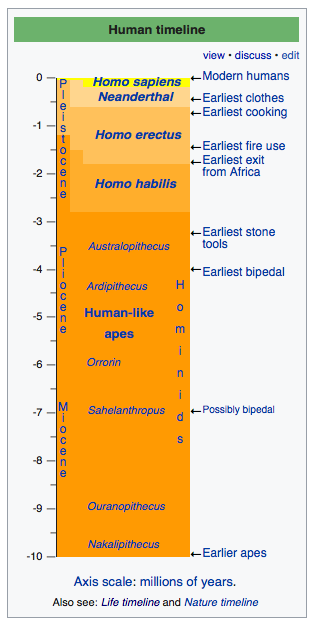
\includegraphics[scale=0.5]{figures/HumanTimeline.png}
\caption{Human Timeline \cite{RefWorks:279}}
\end{figure}

Over that million years, the world economy has been steadily growing, doubling at a measurable rate over an interval that has been decreasing over time. Occasionally a technological or biological innovation takes place that increases the rate at which the world economy doubles. The evolution of the human species to homo-sapiens was one biological evolution. The Agricultural revolution around 5000 years ago was another and the comparatively recent Industrial Revolution
\begin{quotation}
If any large system of interacting parts tends to improve by smooth gradations,
then we should expect systems of systems, with their larger number of
components and interactions, to improve even more smoothly. By this reasoning,
the world economy should improve most smoothly of all. The world economy
consists of the largest number of interacting
parts of any man-made system, and everyone not stranded on an
uncharted island contributes to the improvements in all those parts by using
them. Finally, in each economic era the question of whether growth speeds up
or slows down depends on two competing factors. Deceleration typically ensues
as innovators exhaust the easy ideas --- the low-hanging fruit. But acceleration
also ensues as the economy, by getting larger, enables its members to explore an
ever-increasing number of innovations\cite{RefWorks:120}.
\end{quotation}

The world economy is being transformed from an analogue system of paper transactions based around physical transaction instruments such as contracts, shares, cheques and physical cash to a digital one. The analogue system must be processed in human time frames, evaluated by humans and coordinated by humans. Digital systems function according to programming and are reliable enough to continue processing to deterministic rules, night and day, in computer systems and networks that improve at the speed of silicon, not at the speed of the evolution of the human species or even at the speed of human thought which might develop innovative new algorithms for processing information. Digital systems improve at or above Moores law speeds and the economic growth in the economy which may have seen a doubling of GDP in a generation can be expected to take less and less time as long as the rate of improvement in information systems continues.

\subsection{Velocity of Money}
An important indicator of the overall health of an economy is a measure known as the Velocity of Money. In every economy, money enters the system, is retained in a suspended state during a transaction and is either destroyed through a loss or eventually credited to an account. The speed with which a payee can spend the amount given to them by a payer in a transaction and whether that payment can be passed on in full is vital to a functioning economy. If payments are made that cannot be passed on to other parts of the economy then goods become less valuable, the economy does not grow but stagnates or shrinks and overall benefits to participants in the economy are eroded. It is officially defined as  nominal GDP divided by the Money Stock, the total value of monetary assets available in the economy at a particular time\cite{John2018}, sometimes referred to as M1\index{M1}.

Electronic transaction systems should accelerate the velocity of money through the system. Before electronic transactions, banks and people used financial instruments such as cheques and passbook bank accounts which could only be accessed during bank business hours and updated once a day. In remote and rural areas, the bank would have been a regional bank manager who would visit the local post office or community hall and set up a branch office for the day to allow people without access to a bank to deposit and withdraw money for use in the community.

Money deposited into the community is often spent in the community as, before electronic transactions and modern transportation and logistics networks, it was complicated and time consuming to purchase items in another area and have them brought to the local community. It would be expected that as electronic systems began to reduce the complexity and increase the speed of transactions that  goods and services would be procured in greater volumes than before and could be procured from markets that were further away due to information systems improving the logistics supply chain and making shipping more efficient. This would mean a reduction of money staying in deposit accounts for long periods and would instead mean that funds would be used sooner after being deposited than in a economy based on manual transactions. The economy would grow in size because Australians, rather than being reliant on state or national markets, could source supplies from the cheapest market even if that market were an international one outside Australia. Indeed, it is possible to see the velocity of money did increase in the 1970's and 1980's when electronic banking and Electronic Funds Transfer at Point of Sale (EFTPOS\index{EFTPOS}) was introduced. However, worldwide, the velocity of money began to tail off until today it is lower than it has been for over fifty years. This is especially true in Japan where the national habit of leaving all excess income in post office savings accounts has meant a money supply that is practically moribund for decades and has contributed to the so--called `Lost Generation' where economic growth has been sustained by government spending. Although, in a purely rational system, digital systems may make great improvements possible, these improvements have to be delivered by people enacting economic policies that make trade possible in the first place. In the case of Japan, consumers seem reluctant to release money back into the money supply. In a similar way, the rich seem to be hoarding cash and getting high returns from the digital economy rather than releasing it back into the human economy.
 

\begin{figure}[ht]
\centering
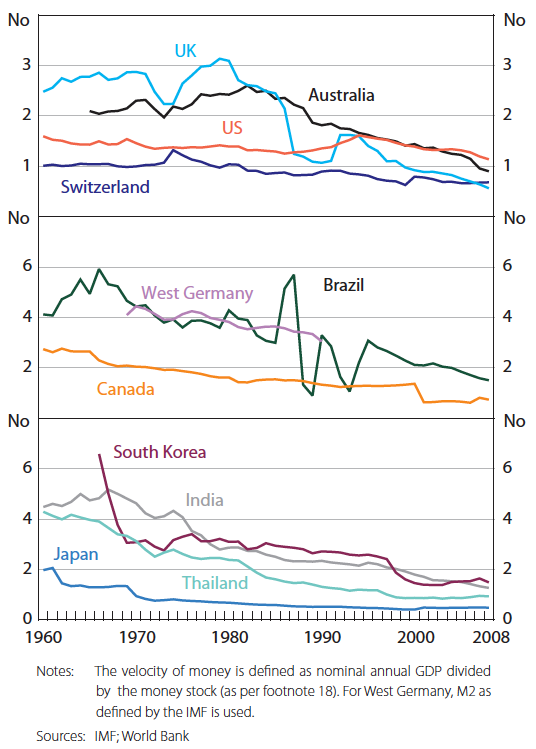
\includegraphics[scale=0.5]{figures/RBAVelocity.png}
\caption{Velocity of Money in the World Economy\cite{RefWorks:251}}
\end{figure}

In other economies, however, another effect is contributing to the slowdown in the velocity of money. It would appear that the rich, are getting richer and that, world wide, even as hundreds of millions of people are lifted into the middle classes and general economic well-being becomes, on average better, the top one percent of the population continue to accumulate earnings far faster than any other group.

This income inequality has been discussed at length by economists Piketty and Reich\cite{Reich2014}. Piketty suggests that the global financial crisis (GFC) may have been inevitable given the rise of inequality in the United States.

\begin{quotation}
In my view, there is absolutely no doubt that the increase of inequality in the United States contributed to the nation's financial instability.  The reason is simple: one consequence of increasing inequality was virtual stagnation of the purchasing power of the lower and middle classes in the United States, which inevitably made it more likely that modest households would take on debt, especially since unscrupulous banks and financial intermediaries, freed from regulation and eager to earn good yields on the enormous savings injected into the system by the well-to-do, offered credit on increasingly generous terms\cite[pp. 372-373]{Piketty}.
\end{quotation}

 

It is tempting to look a current measures of income inequality and point to the several measures that show that a small percentage of the population is retaining the majority of the money in the economy and, through that accumulation, is becoming even more wealthy. 

It would appear that a small number of individuals are corralling their earnings in illiquid investments and bank accounts and reducing the money supply. Restricting the velocity of money would seem to both reduce the number of positive cycles of this money through the economy and therefore reduce the number of times that it could be spent on productive purposes as well as reducing the number of participants who could share its benefits. This constraint would appear to benefit urban areas as it would be assumed high income earners would cluster to economic, cultural and transport network nodes. 

An analysis of data from the ABS, however, reveals that some remote and very remote areas appear to have enough high income earners that they are, on average, better locations economically than some urban areas. In 2015, the Median Income in Sydney's Balmain, in a Major Cities area for example was AUD72,591 compared to the national Median Income of AUD44,940. However there are some Remote areas such as the Ashburton area in Western Australia where the Median Income is AUD93,902. The Outer Regional communities of Moranbah in Queensland with a median income of AUD80,945 and Umbakumba on  Groote Eylandt, NT with a median income of AUD62,027 are examples of communities that owe their wealth to the mining industry.
%http://www.sbs.com.au/news/map/regional-variations-in-income
%http://www.abs.gov.au/AUSSTATS/abs@.nsf/DetailsPage/6524.0.55.0022011-2015?OpenDocument


\subsection{Effect of location on velocity of money}
If cash is not easily accessible through online transaction network; if it has to be downloaded from a branch or a machine before its packetised value can be used in the local economy then its ability to perform as an engine of growth and creation is curtailed and it instead savings are hoarded or withheld because the availability of future money is constrained by when the next journey must be taken to an ATM or branch. In urban areas this can be mere minutes or hours away but in remote and regional areas, each monetary download may be days or weeks apart.

\begin{figure}[ht]
\centering
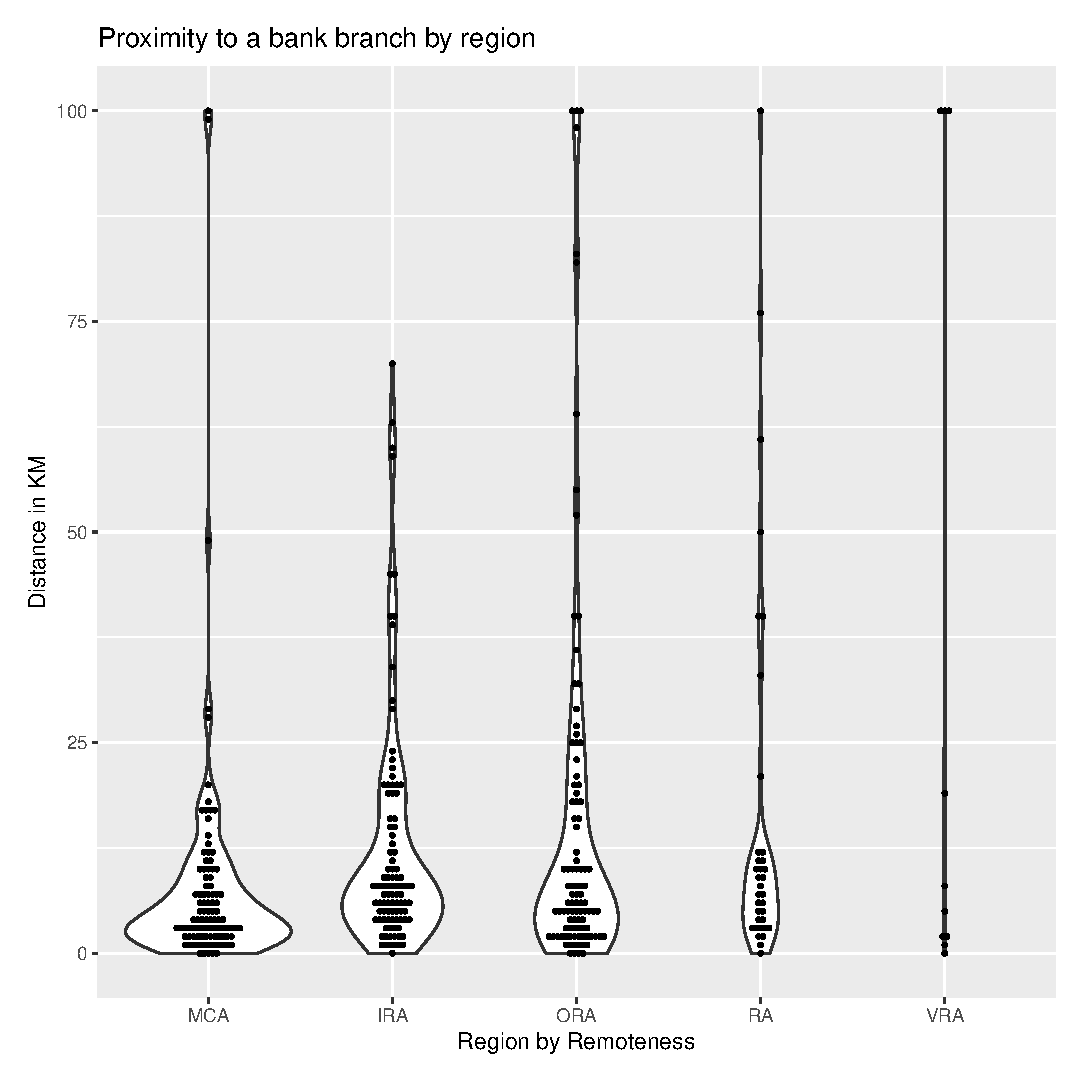
\includegraphics[scale=0.5]{figures/VChart07-Proximity2BankBranch.eps} 
\caption{Proximity to a Bank Branch by Region} \label{fig:VC07BankProxRegions}
\end{figure}

In my survey(Figure \ref{fig:VC07BankProxRegions}, I asked the question about proximity to a bank branch expecting that people in more remote areas would have to travel more than 20 kilometres in some cases to access branch services but this did not appear to be the case for respondents to this survey. I remember, as a child, my father driving to a town 25 kilometres away over flooded roads in order to make a home loan payment on time, something that would not be necessary with phone banking, internet banking or today's electronic transfers and direct debits. It was necessary then, in the 1970's, because the transaction was in cash.

Almost all the respondents to this survey were able to find a bank branch within twenty kilometres of their location. Banks and doctors seemed to be similarly close to the survey respondents, possibly because both congregate in the same sized towns in Remote and Very Remote areas. I posed this question in the survey due to overseas experience with so-called `Banking Deserts' in the UK, USA and New Zealand. Banking Deserts echo the concept of `Food Deserts' where there may not be a grocery store within a comfortable distance of the population. In Banking Deserts there may be no bank branch, ATM or EFTPOS capable merchant within a reasonable distance of the population.  I found that The New York Federal Reserves cites a census region or `tract' with roughly 4000 people in it and with no bank branches within ten miles (16 kilometres) of the centre of the tract. In my survey (Figure \ref{fig:VC08ATMProxRegions} I found that, once again, the majority of the respondents, regardless of remoteness, were within 25km of an ATM and would have been within the 16km that is regarded as being within range of an ATM and therefore not in a banking desert. Although the survey data does not confirm this assumption, there is evidence that accessing banking services is becoming more difficult for people in remote areas.
\begin{figure}[ht]
\centering
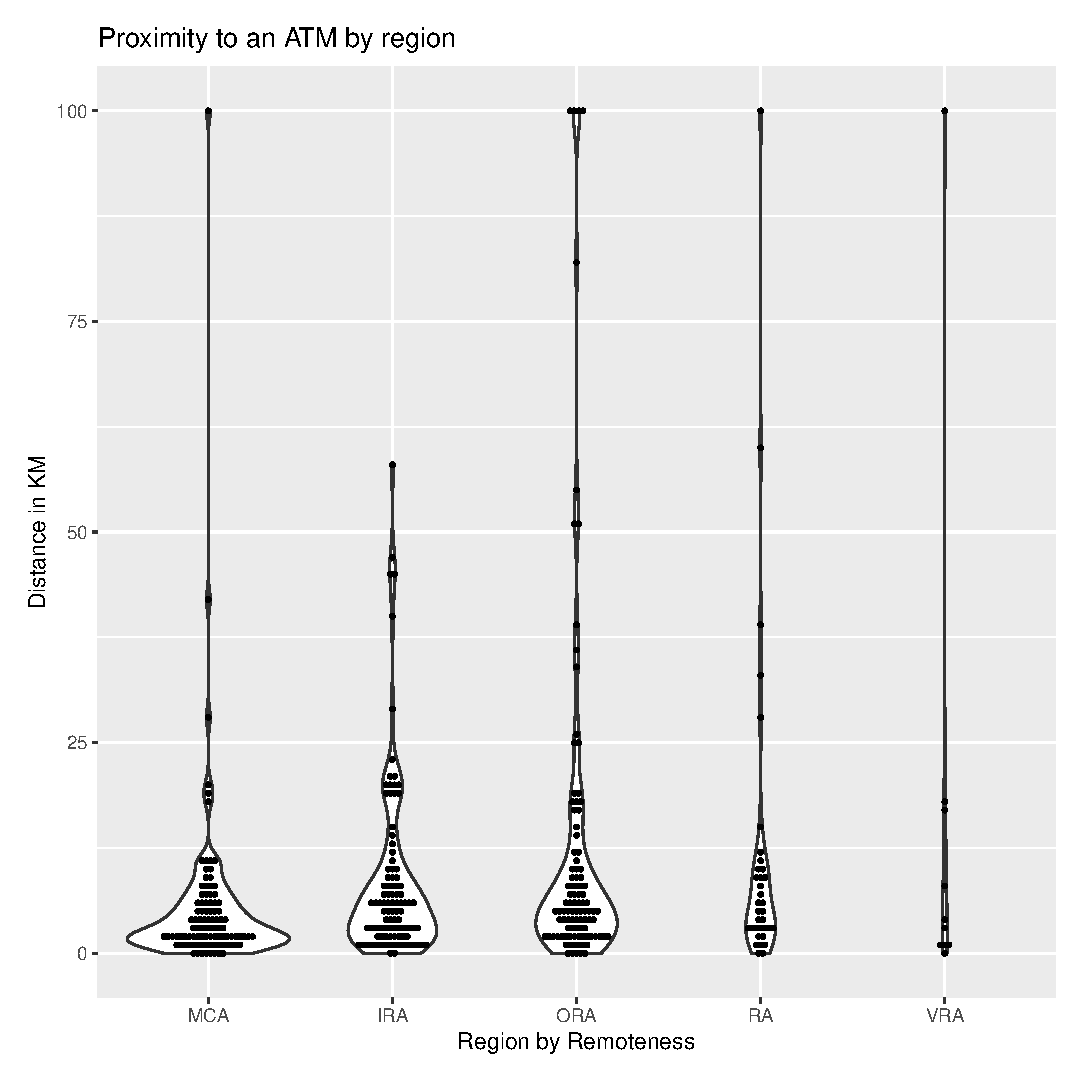
\includegraphics[scale=0.5]{figures/VChart08-Proximity2ATM.eps} 
\caption{Proximity to an ATM by Region}\label{fig:VC08ATMProxRegions}
\end{figure}

In the UK and the USA, large scale branch closures have created many areas where there may be no in person banking service and only the limited services of an ATM are available. In the US, there have been thousands of bank closures since the Global Financial Crisis (GFC) \index{GFC} in 2008 when the banking industry had opened 100,000 branches. Since then, 10,000 branches have been closed leaving large towns with over 4000 people without any bank branches.\cite{RefWorks:395} In the UK, the bank branch network has been shrinking since the early 1990s with the effect that most small businesses have been starved of credit while large businesses, congregated in Major Cities, have been the major beneficiaries. The UK lacks a large scale credit union base since its banking system originally evolved from a highly decentralised branch network which prevented credit unions from taking hold\cite[p332]{RefWorks:402}. Although the retreat of large bank branch networks from regional centres presents an opportunity for non-bank lenders to originate business in these areas, there is more evidence of concentration than of decentralisation in the banking sector in the UK and that this is having a negative impact on lending to small businesses which in turn is contributing to a sub-optimal economic recovery for the UK as a whole\cite[p55-56]{RefWorks:403}.

Business access to credit in negatively affected by its distance from a bank branch with those businesses closer to the branch having easier access to credit than those that are further away. Personal relationships between the lender and the borrower seem to be important for small-business access to credit where mortgages are approved by a more rigid set of credit scoring rules and are not as influenced by proximity to a branch\cite{RefWorks:394}.

Branches staffed by people living in and holding a stake in the local community is important to the economic well-being of an area. Access to ATMs may not always give bank customers access to cash. A British report on bank branch closures found that ATMs were unreliable as a means of obtaining cash and were often sited in inconvenient locations that had more to do with inexpensive rent for the ATM owner than with the convenience of the account holder \cite[p16-18]{RefWorks:397}.

The New Zealand government privatised the national Post Office bank before selling it to ANZ but found, after also selling off the Trustee Savings Banks, the Bank of New Zealand and Postbank to Australian Banks that they had to recreate a national banking network with the government forming `kiwibank' to ensure a network of 221 bank branches would continue to operate when ANZ closed many non-urban branches\cite{RefWorks:377}.





Automated Teller Machines (ATMs)\index{ATM} are important in remote and very remote communities because they are operational every hour in the day and every day in the year. For an area that may have irregular branch hours, they may be the only source of cash outside of business hours. Originally designed to not only provide after-hours service but to replace regular bank tellers with robots that didn't tire, didn't require holidays, pay rises or performance management, ATMs have grown from being merely a cost saving measure to being a revenue raising machine that outstrips the profitability of a regular teller. Since the Reserve Bank of Australia (RBA) reforms of 2010, most Australian banks added a direct fee of \$2.00 or more to each  transaction that is made on an account that is not that of the ATM operator, a non-own bank fee. Before this, fees were passed between the banks as a fee for funds interchange but the RBA ruled that these fees should be abolished.  In 2017, this fee was abolished by the four largest banks for transactions on their own ATMs\cite{RefWorks:458} in a decisions that they admitted would forego AUD500million in fees. Removing fees on major bank ATMs though has not affected those ATMs that are not owned by major banks which represent much of the challenge for regional and remote banking users who must rely on convenience store ATMs and branch ATMs owned by building societies and other institutions who still apply this \$2.00 fee or a higher one. For example, `'\ldots{}while [National Australia Bank's] announcement covered its 1500 machines, a further 3100 NAB-branded rediATMs --- located in pubs, clubs and convenience stores, and a range of other places --- will continue to charge fees.\cite{RefWorks:457}''

\begin{figure}[ht]
\centering
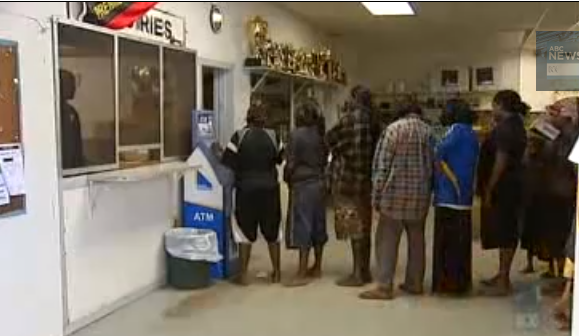
\includegraphics[scale=0.5]{figures/ATMLine.png} 
\caption{People waiting to use an ATM in a Remote Community\cite{RefWorks:378}}\label{fig:ATMLine}
\end{figure}

The RBA's 2010 enquiry discovered some people were spending up to 20\% of their income on ATM fees.\cite{RefWorks:379} 
Fees were abolished in May 2012 on 73 Remote communities but these fees still exist for some ATMS in non-remote communities.
Shopkeepers sometimes require customers to use their ATMs rather than Electronic Funds Transfer at Point of Sale (EFTPOS)\index{EFTPOS}. Fees are charged at some ATMs for even checking a balance. When customers are expecting a deposit, for their salary or government benefit for example, they may check their balance more frequently. Balance checking can sometimes be 20\% of a person's costs for the month as no other means of checking electronic transactions such as mobile banking may be available due to poor mobile service coverage or the inability to use the banking `app' to do so. With no other access to cash in some remote and very remote areas, there is sometimes no way to retrieve a government benefit payment without being charged up to \$10 per transaction.\cite{RefWorks:378}


\subsection{Prioritising the internet --- what is the weekly spend?}
The next five survey questions were designed to find out how much is spent on accessing the internet, talking and texting and entertainment delivered over channels similar to the internet.  Like using games consoles, cable television and some internet and mobile communications use is discretionary and can represent a large expense if household income is low. 

Like video game entertainment, the cost of broadband and talking and texting on mobile and fixed line telephones has fallen sharply over the last two decades. Where mobile phone calls and texts were once a large part of monthly household income expenditure, the prevalence of mobile phone bundles where texts and calls are unlimited has meant that expenditure on communications is more predictable and manageable as a share of regular household expenditure than when a single phone long distance phone call could cost as much as a monthly phone bill does now.
\begin{figure}[ht]
\centering
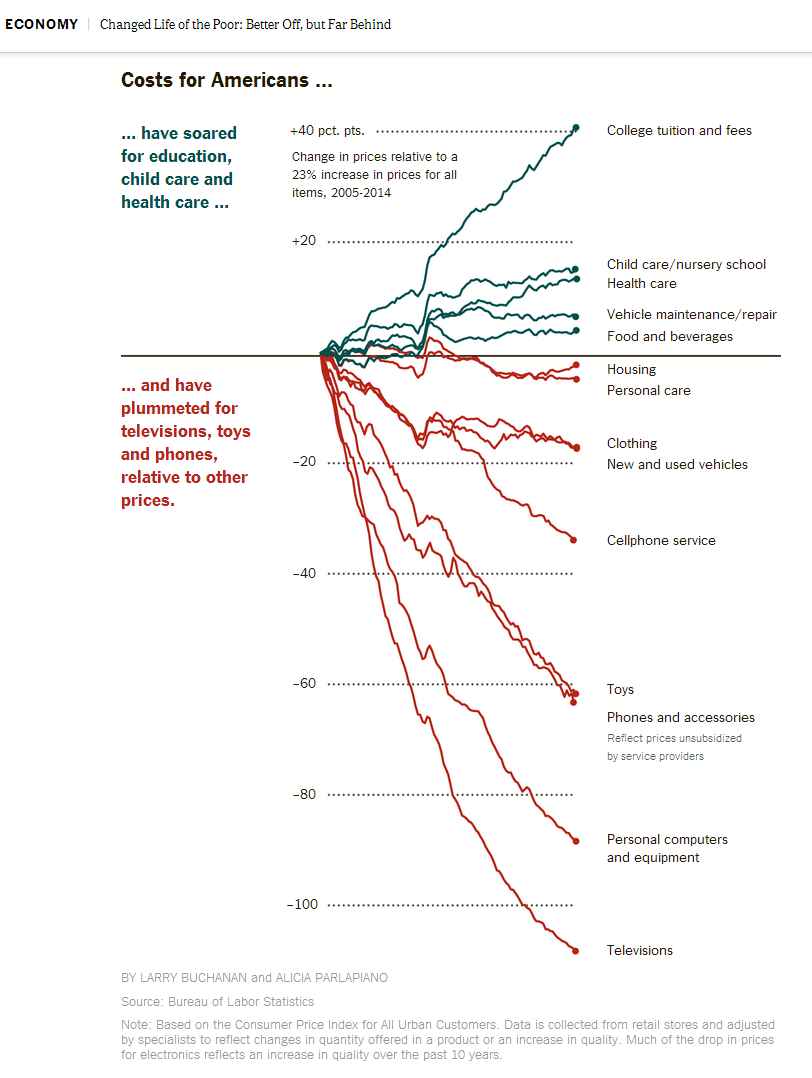
\includegraphics[scale=0.4]{figures/ChangedLifeOfThePoor.png} 
\caption{The plummeting cost of ICT, Toys, Clothing and Vehicles\cite{RefWorks:323}}\label{fig:ICTCosts}
\end{figure}

Very few people spend more than AUD\$10 per week on a home telephone line with the majority in all regions spending nothing at all. This may be because they share the phone with another person who pays the bill or that they do not have a land line phone at all as is becoming more common. Over 30\% of Australians have no fixed line telephone at home.\cite[p15]{acma2016} and with more than 80\% of Australians owning one or more mobile phones, there are more phones in Australia than there are people. In fact, there are more second hand phones in Australia than the  Australian population with over 25.5 million discarded but not recycled by their owners.\cite{RefWorks:405}
\begin{figure}[ht]
\centering
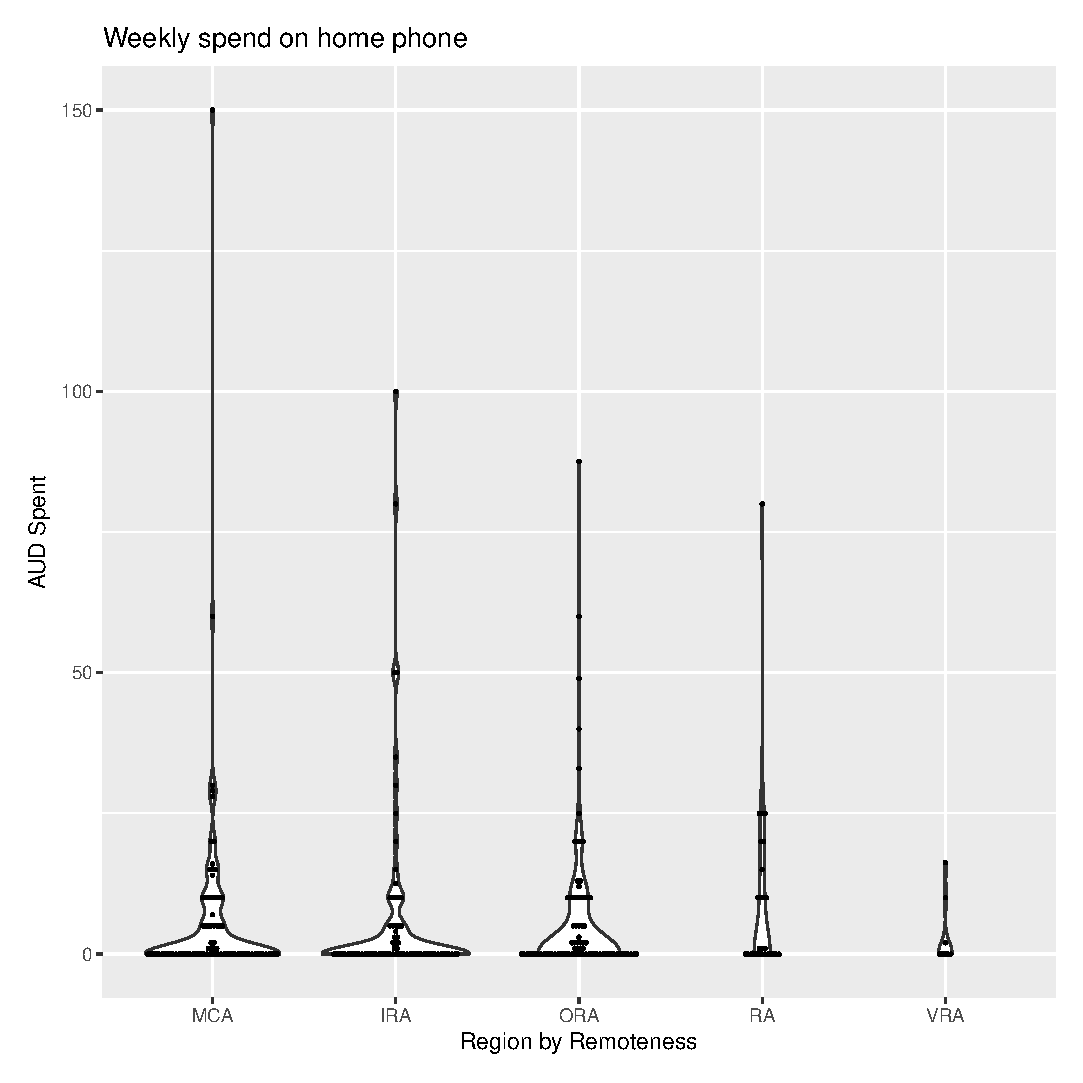
\includegraphics[scale=0.5]{figures/VChart11-WeeklySpendHomePhone.eps} 
\caption{How much is spent on operating a home telephone by Region}\label{fig:VC011HomePhoneSpendRegions}
\end{figure}

If the home phone line has collapsed as a way of staying in touch, are respondents spending their discretionary income on entertainment or mobile phone or broadband via ICT?

Another area of household spending that is being transformed by the internet is entertainment, especially subscription television. 90\% of US households and 60\% of UK households watch subscription television\cite{RefWorks:406}.  Australians are less likely than other countries to watch subscription television with subscription television deployment essentially static over the last decade at around 27\% of households. This represents 5,309,000 viewers of linear subscription television. It seems that regardless of area, most of the respondents in my survey (Figure \ref{fig:VC012CableSpendRegions} spend next to nothing on subscription television every week. While they have never enthusiastically watched subscription television,  Australians have embraced \acrfull{svod}.\index{SVOD}  Since SVOD became available in Australia in 2014, more viewers have access to it than have access to linear subscription television. By 2016 the audience size of 5,595,000 Australians, that meant over 300,000 more viewers watch SVOD services such as Netflix, Stan and YouTube~Red, as well as the SVOD versions of linear subscription television channels Foxtel Now and Fetch TV than watch traditional subscription television\cite{RefWorks:407}.


\begin{figure}
\centering
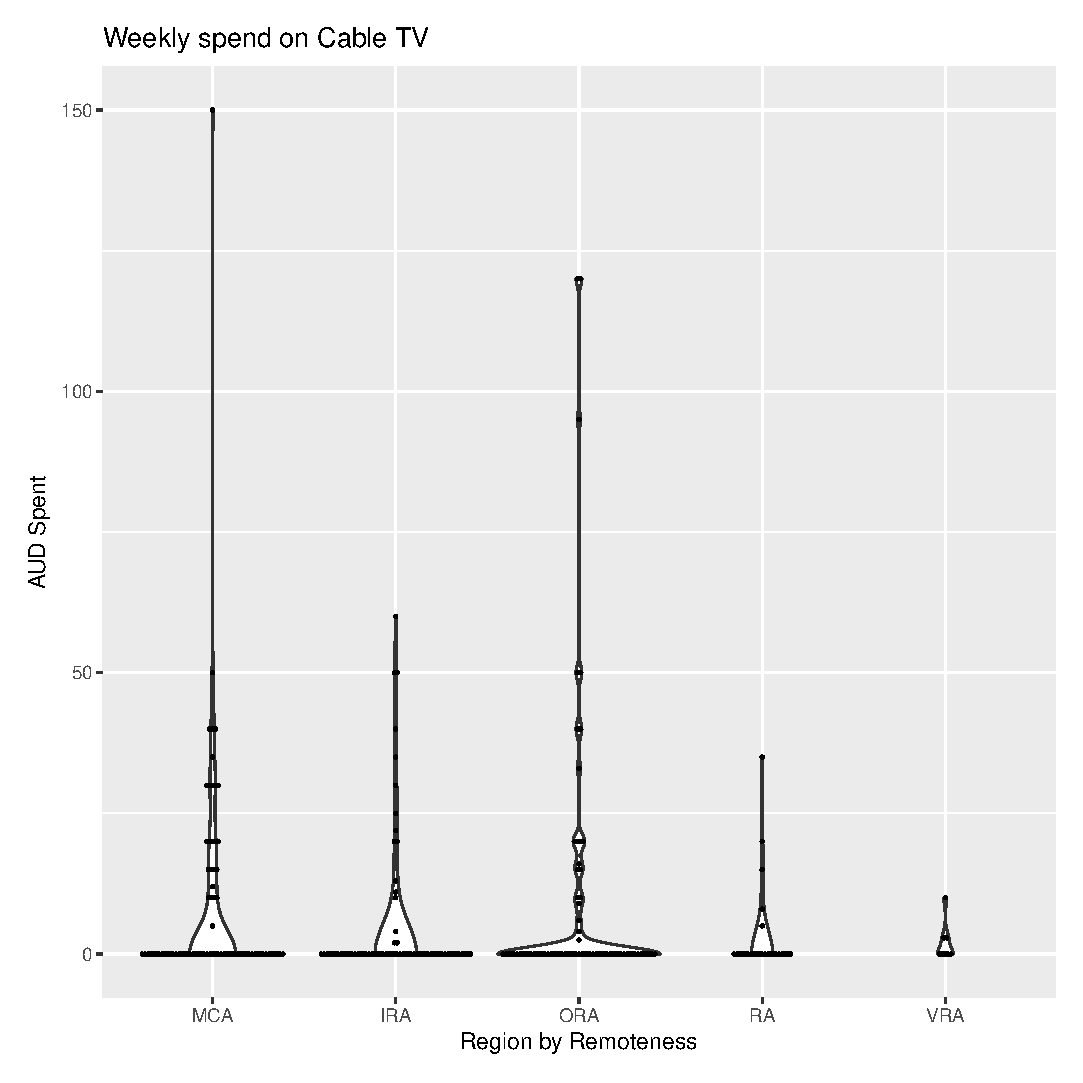
\includegraphics[scale=0.5]{figures/VChart12-WeeklySpendCable.eps}
\caption{How much is spent on Cable TV by Region} \label{fig:VC012CableSpendRegions}
\end{figure}
In Major Cities and Inner Regional Areas, there were a number of respondents who spent up to ten dollars a week on Cable TV but this fell off to less than five in Outer Regional, Remote and Very Remote regions, possibly because most cable infrastructure was installed in Major Cities and Inner Regional Areas long ago during the first wave of the Foxtel and Optus network building effort.

Since more viewers have been added to the SVOD platform in two years than were added in the 25 years before, it may be assumed that the internet will be the prime delivery method for subscription entertainment in the future\cite{RefWorks:407}.
\begin{figure}
\centering
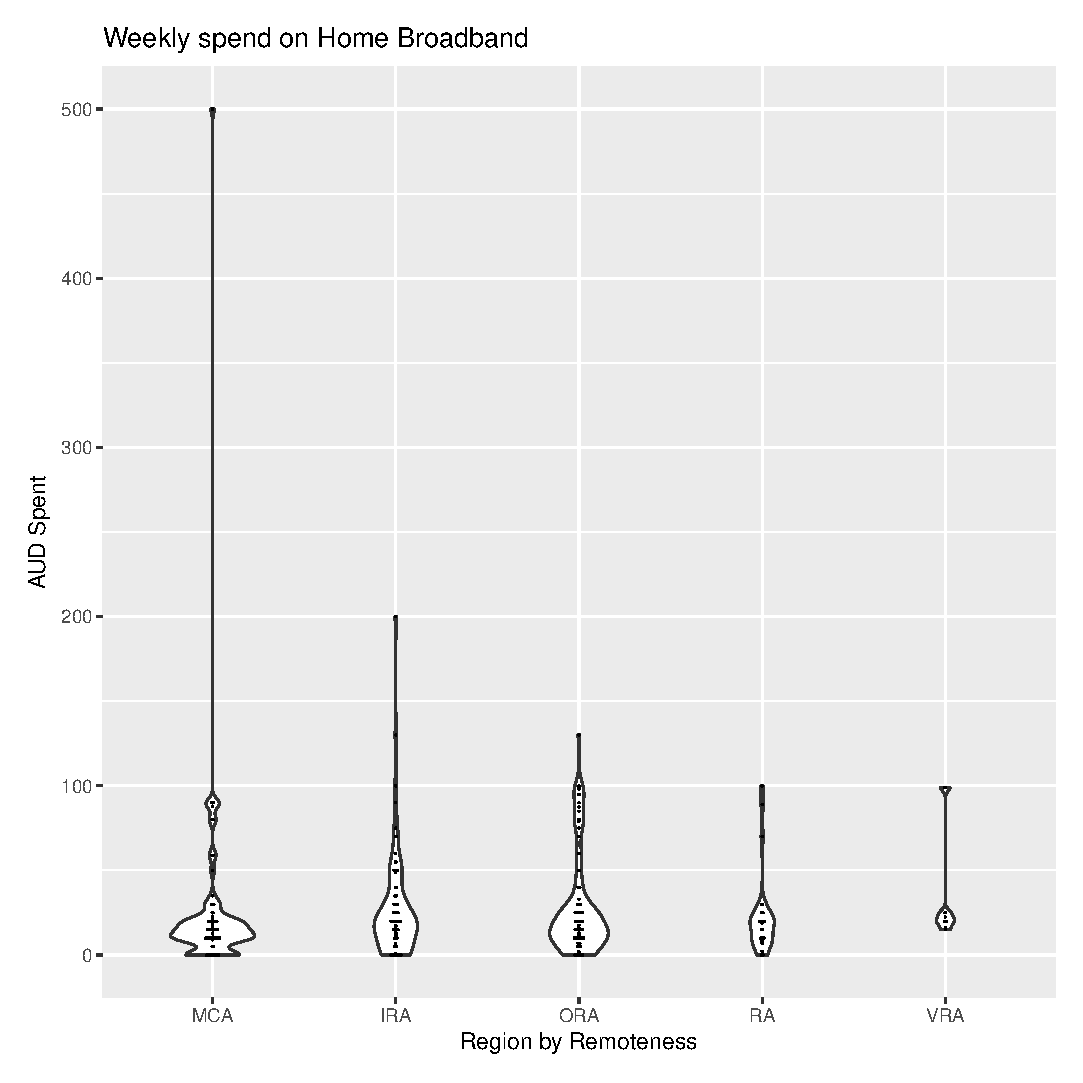
\includegraphics[scale=0.5]{figures/VChart13-WeeklySpendHomeBroadband.eps}
\caption{How much is spent on Home Broadband by Region} \label{fig:VC013HomeBroadbandSpendRegions}
\end{figure}
While the internet may be the way most people watch television in the future, accessing the internet is not free.  In my survey, most respondents spent under \$50 per week (Figure \ref{fig:VC013HomeBroadbandSpendRegions}). Respondents in Very Remote Areas all spent something on internet access while some respondents in other areas did not spend anything and were presumably dependants using another person's connection or a mobile connection. Average spend on telecommunications per household in Australia has remained at around \$2000 per year or \$38 per week for several years even as it has fallen in other countries. Australia is now the ranked at 57 in fixed internet affordability with the average cost rated as USD46.7 in Purchasing Power Parity (PPP)\index{Purchasing Power Parity} terms. Australia is ranked at 100 on the World Economic Forum's list of 137 countries below countries such as Vietnam, which has the most affordable fixed broadband, Malaysia, Indonesia and China\cite[p27,229]{RefWorks:412}. Australia's position in world rankings for internet affordability continues to decline even as some of the most remote areas of the world are getting internet access for the first time. 

Remote Australia resembles a developing nation in respect to the provision of internet services. Mobile, fixed wireless or satellite service is favoured over fixed line service because providing fixed lines to a large geographic area is uneconomical outside of a densely populated area. 

\begin{figure}[ht]
\centering
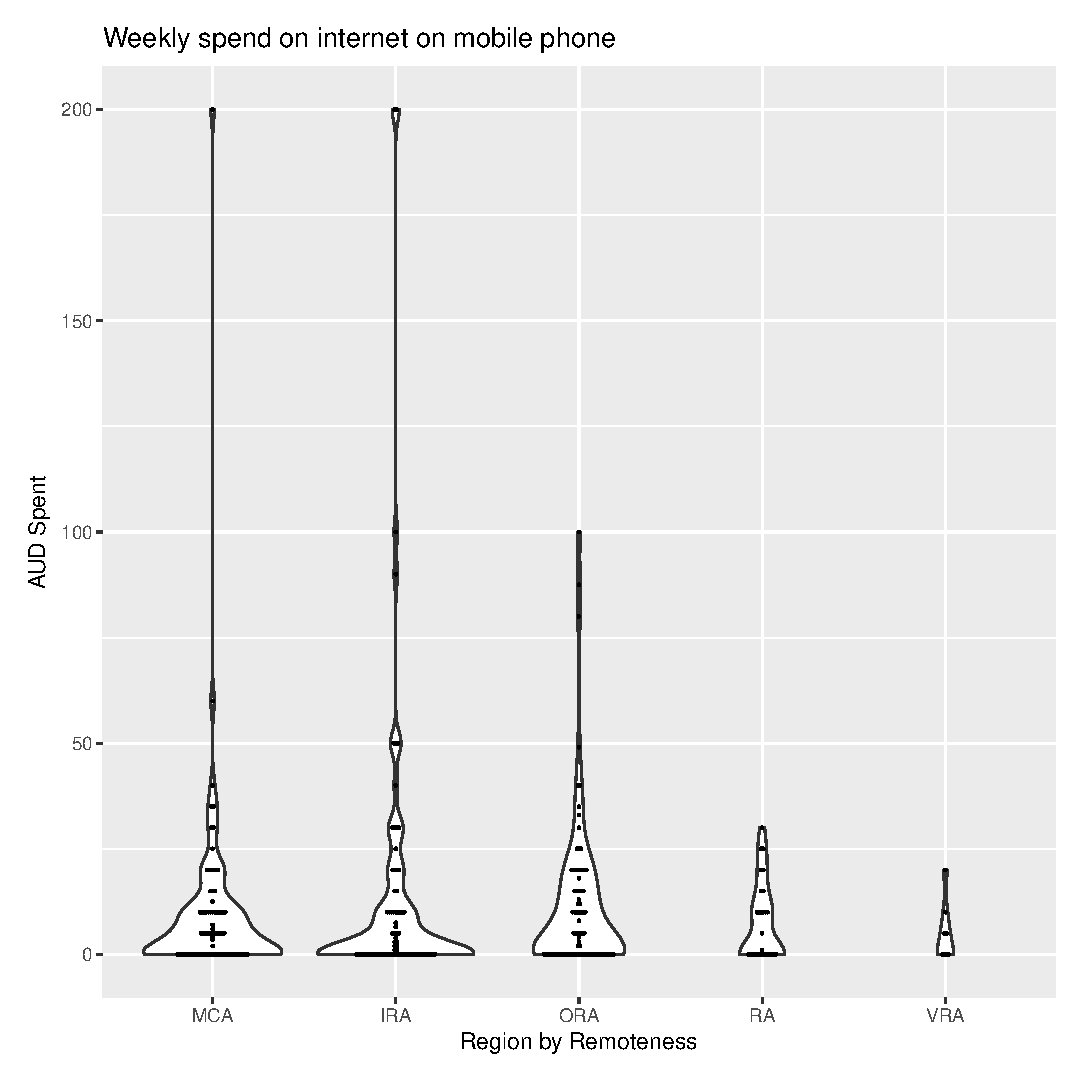
\includegraphics[scale=0.5]{figures/Vchart14-WeeklySpendMobileInternet.eps}
\caption{How much is spent on a Mobile internet by Region} \label{fig:VC014MobileInternetSpendRegions}
\end{figure}


Mobile internet is valuable to Australians and especially valuable to Australians in non-urban areas that are not well served with fixed line connections. In 2011 mobile broadband was up to 1333 times more expensive than fixed but this situation has improved. Telstra are offering mobile broadband plans of 100GB for \$199 or \$1.99 per \acrshort{gbyte} whereas Optus market a mobile broadband solution which uses a fixed WiFi base-station that also provides telephone services for \$70 per month and includes 200GB of data or \$0.35 per GB\cite{RefWorks:413}. Even this price is expensive compared to the cost of Unlimited broadband plans on fixed lines where the price per gigabyte is difficult to calculate because few carriers classify the total number of gigabytes a consumer is allowed to download in a month before they apply a `fair use' policy and `shape' or limit their download speed to prevent them using more data than the company can afford to provision. If Telstra's 1000GB fixed line plan for \$90 per month or \$0.09 per GB is taken in a comparison with their cheapest mobile broadband plan of 100GB at \$199 per month or \$1.99 per GB then mobile service from Telstra is still 22 times more expensive than fixed broadband while being limited to one tenth of the monthly download quota.

This question was asked to check research that had been published by \acrshort{birrr} that showed Rural, Regional and Remote internet users were charged very high prices for mobile broadband which they were forced to use for lack of an alternative. \acrshort{birrr} indicated that 71\% of their survey respondents paid between \$6.00 and \$10.00 per \acrshort{gbyte} of data for up to 30 gigabytes per month with one respondent paying \$20 per gigabyte to receive 14GB per month at a total cost of \$280 per month\cite[p19]{RefWorks:212}.  If the price per gigabyte of mobile broadband is so variable it may be because the respondent is on an old plan that they have not updated or is on a plan they cannot change because the plan was bought with phone hardware and the respondent has a contract and cannot change it. The discrepancy may also be due to respondents being unable to understand different cost structures of plans to get the cheapest deal or that the cheaper vendor does not offer service in their area.

Respondents to this thesis' survey (Figure \ref{fig:VC014MobileInternetSpendRegions}) in Remote and Very Remote Areas indicated that the did not spend over \$100 per month on mobile internet with the majority spending under \$25 per week. Surprisingly, at least one respondent in Major Cities and Inner Regional Areas indicated that the spent \$200 per week on mobile internet which would involve a spend of around \$800 per month. Most respondents in all categories spent within \$25 per week or \$100 per month on mobile internet and respondents in Major Cities and Inner Regional areas on average seemed to spend less than respondents in Outer Regional Areas.


\begin{figure}
\centering
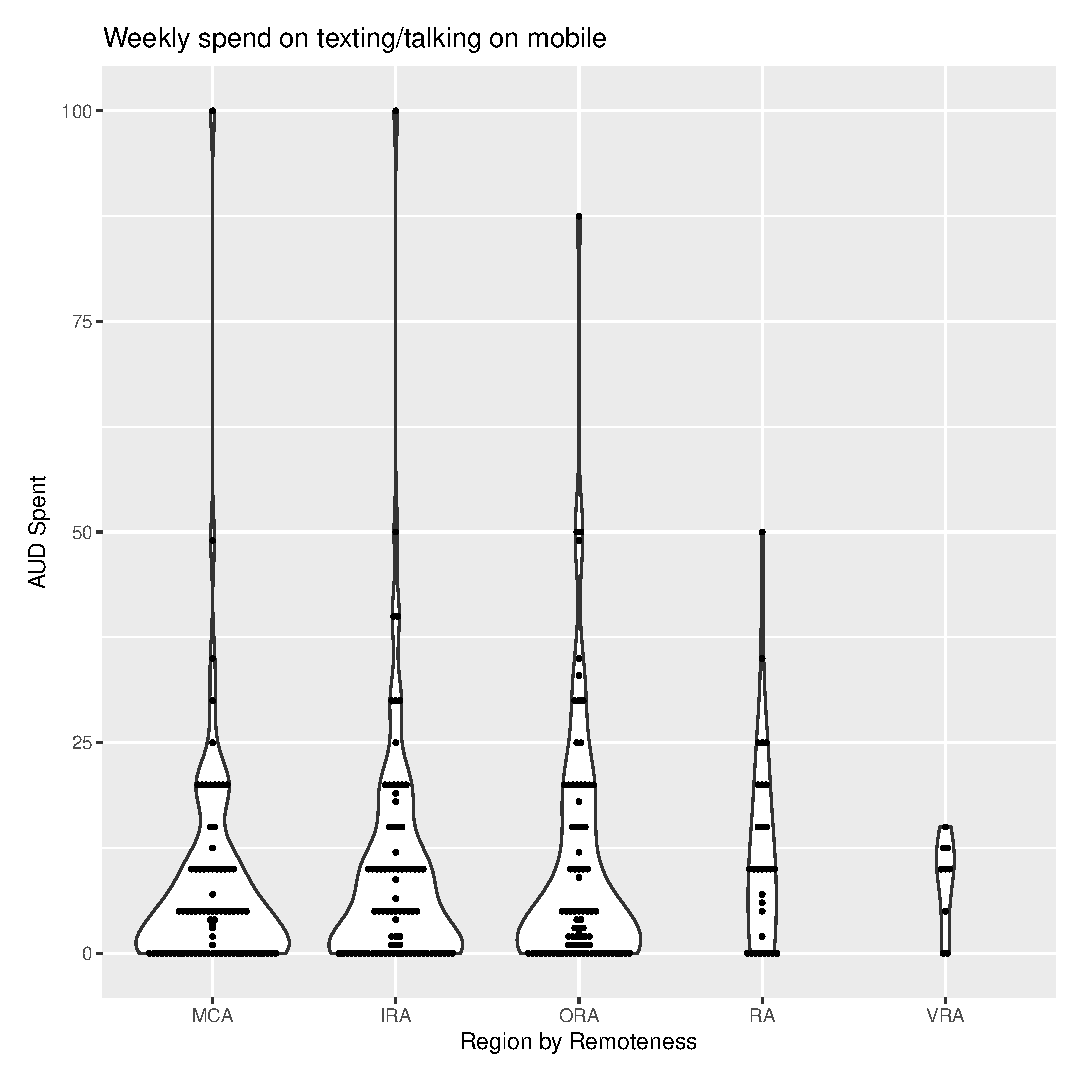
\includegraphics[scale=0.5]{figures/VChart15-WeeklySpendTalk.eps}
\caption{Weekly spend on talk/texting phone plans by Region} \label{fig:VC015WeeklySpendTalkRegions}
\end{figure}



\subsection{High Speed Transactions}

Australia is well situated to take advantage of the new, hyper connected machine based transaction economy. We have one of the largest superannuation industries in the world, a highly centralised banking sector that is centred around a government backed ''four pillars'' strategy and a banking and finance sector that has been heavily computerised since the first mainframes. Unfortunately it is at the mercy of some basic laws of physics when it comes to its desire to become a centre for banking world wide or even in our Asian region. The velocity of money and the speed with which money can be moved from one place to another in the economy has been demonstrated above to be a significant driver to increasing overall economic well-being. This effect is magnified in the machine world where transactions, instead of taking days take seconds or milliseconds. This increases the effective amplitude of the benefits and damage to the economy through successive transaction iterations. Whereas, in the past, it may only have been possible to trade a stock once every few minutes, it is now possible to do so thousands of times a second. Entities still need to come together in an exchange to make trades which is why regional exchanges such as the Australian Stock Exchange and exchanges such as the New York Stock Exchange and the London Stock Exchange are such important institutions. In the past they provided a place for individuals to come to buy and sell stocks in an 'open cry' environment where people bought and sold from other people by shouting orders at them. With the automation of these exchanges the scale of the transactions and the speed of those transactions increased dramatically. A generation ago, every Australian state had its own stock exchange. These were amalgamated into the Australian Stock Exchange in 1987\cite{RefWorks:258}.

Inside the exchange, stocks can be traded with almost no latency. Orders are filled on the stock exchange servers with no communications latency if the buyer and seller are both accessing the server over the same network. If a trader is manually entering a trade on their terminal in Melbourne or Brisbane, there will be little difference in the delay between them since it is limited by the speed that an individual can key in the order. If, however, financial institutions allow programs to monitor stock prices and information feeds and make the trades on their behalf, no such limitation exists and stocks can be bought and sold by whoever can put the trade through first. This produces a race to remove the delays between networks but there is no substitute for moving the stock broker's computer closer to the stock market's servers. If a broker in Western Australia is executing trades in Sydney, they face a Round Trip Time, the time required for a request to get to the stock exchange and then return with an message of success or failure, of  around 106 milliseconds. 

Australia has aspired to a primate role in the global financial system in Asia. The \textit{2014-15 Australian Cities Accounts} report says that

\begin{quotation}
Sydney and Melbourne are driving the national economy. Sydney contributed 30.3 per cent of all Australian Gross Domestic Product (GDP) growth in 2014-15. While driven by Financial services, its growth was broad based with a range of industries contributing to growth. The city's role as a global financial hub has allowed it to tap into the benefits of stimulus programs undertaken by central banks around the world\cite{RefWorks:278}.

\end{quotation}

Australia is, unfortunately, at almost the edge of every major financial network in the world. At the speed of light, Sydney is tens of milliseconds away from other financial capitals compared to similarly qualified cities in Asia such as Singapore, Shanghai and Tokyo, all of which also have aspirations for being transaction hubs in the global economy. When communication was by voice or even teletext or telegraph, this did not matter but now an order to buy or sell may take place in a few thousandths of a second and the time taken for that transaction to go from the buyer to the seller has to take in several real world limits.

Although transactions are presumed to take place at the speed of light, the speed of light through fibre optic cable is actually around 70\% of it's speed in a vacuum. This means that a packet of information theoretically travel from Sydney to London and back again in 610 milliseconds (305 milliseconds each way). Human visual and auditory acuity can notice as little as 5 milliseconds delay and natural interaction with a party on the other end of a telephone conversation becomes difficult above 10 milliseconds latency so when the latency is over half a second it is beginning to become necessary to employ unnatural communications styles which we are all familiar with where one party talks and the other listens until it is their turn to speak. 

In high frequency transaction environments, brokers who are outside the latency threshold of the majority of other brokers are at a disadvantage. Trades can be executed by other parties closer to the exchange before their order to buy or sell has even reached the exchange server. In some exchanges, brokerages are paying to have their servers moved from their own data centres to be collocated in the same data centre as the exchange servers. Some even pay to ensure they are on the same network switch as the exchange server to further minimise latency for trades. 

There is evidence that High Frequency Traders (HFTs) who can move faster than Other Traders(OT)s can exploit several strategies to out manoeuvre or overwhelm slower traders.

\begin{quotation}
If HFTs have the ability to detect large orders of OTs, then they can prey
on them. This raises OT transaction cost and leads to slower price discovery. The evidence
suggests HFTs are able to predict OT orders and to back-run on long-lasting informed orders of
institutional investors. The institutional investors experience higher transaction costs when this
happens\cite[p12]{RefWorks:280}.
\end{quotation}

\begin{figure}
\centering
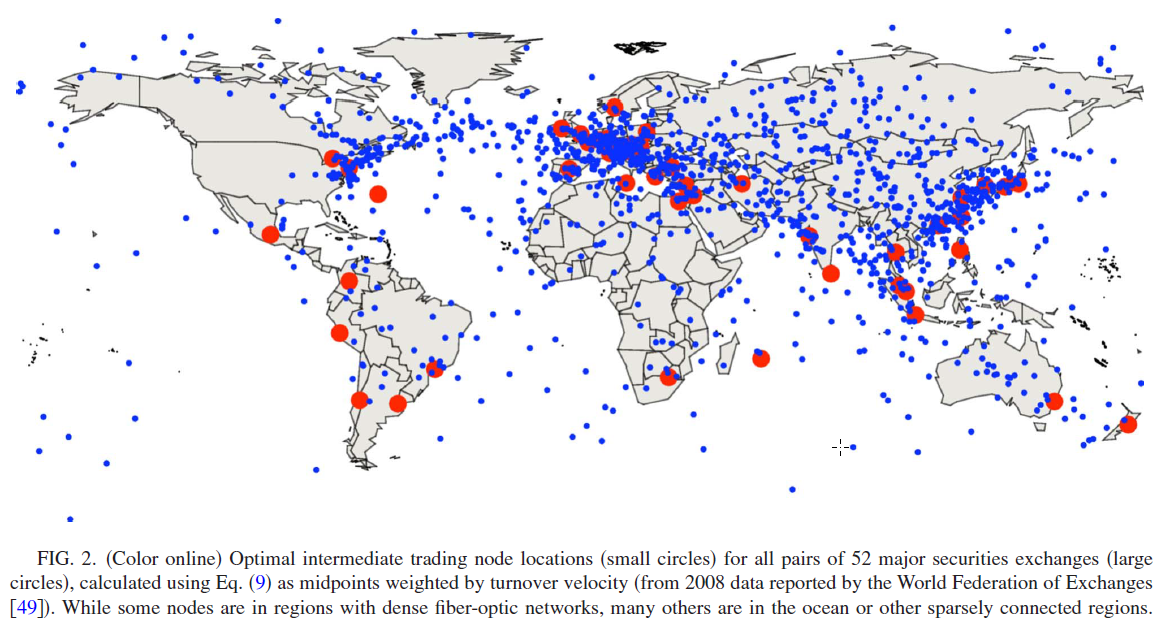
\includegraphics[scale=0.5]{figures/RelativisticStatisticalArbitrage.png}
\caption{Relativistic Arbitrage for City Pairs between major Finance Centres\cite{RefWorks:281}}
\label{relativistic}
\end{figure}

Australia's geographic disadvantage means that it cannot effectively compete in the intense HFT markets of global financial centres such as New~York, London and Tokyo but these are not the only markets and not the only way to compete in the high speed world of HFTs. There are some situations where Australia's position gives it an advantage in financial markets, even in remote and very remote locations. At points on the Earth that are equidistant between large financial centres, Figure \ref{relativistic}, it is possible to exploit arbitrage opportunities between these centres from a point between them that would provide a trader with a better position, from a HFT/latency point of view to if that trader was based in one or the other or both financial centre.

\subsubsection{Real Time Gross Settlement system}
The Reserve Bank has been at the forefront of real time transaction processing since 1998 when it set up the Real Time Gross Settlement (RTGS) System. This system illustrates issues with a low velocity of money in the economy. Before the RTGS system, each bank sent a single payment in fulfilment of all their obligations to another bank in a single transaction every day at 9am Sydney time. All transactions on all accounts were accumulated into this single daily settlement which, as the economy grew over time, amounted to a very large systemic risk if any one bank failed to make their settlement obligations on a single day. By allowing real time settlement of accounts interbank, the Reserve Bank lowered a significant systemic risk in the economy\cite{RefWorks:256}.

This risk has been lowered between banks for high value transactions. This risk still exists for smaller transactions that occur between individuals and small company transactions. These are settled on a different system that still accumulates all transactions to an account that is identified by a bank branch 

\subsubsection{Clearing House Electronic Sub--register System}
The Clearing House Electronic Sub--register System (CHESS) was developed in the late 1980s to minimise a similar risk in the daily trade in securities and other financial products. 
\begin{quotation}
The need for establishing a more efficient system was highlighted during the 1986/87 ``bull'' market. Settlement backlogs, caused by failure to deliver promptly, stemmed the free flow of funds between industry participants and between them and their clients, as well as raising concerns about counter--party risk\cite{RefWorks:255}
\end{quotation}

These systems have all been implemented to remove risk from the banking and finance system in Australia and diminish the negative consequences to individual parties in that system.



\subsubsection{The Reputational Economy}
The idea that having a good reputation is objectively a good thing is part of our culture but how does reputation affect the economic well-being of a community. All Australians already have an economic reputation that is dictated by their credit score as determined centrally by the Credit Reference Association [reference] but there are other ways in which Australians can be disadvantaged by their location.

In the science fiction novel, \textit{Down and Out in the Magic Kingdom}\cite{RefWorks:380}, Cory Doctrow posits a future society where all basic needs are met, people are essentially immortal and can have their memories restored from backup into cloned bodies after death from misadventure. Limitless energy comes at no cost and people are not limited by the scarcity of resources. The primary pursuit in this world is the acquisition of a fictional currency known as Whuffie that indicates a person's reputation within society. Individuals gain Whuffie through the perception of their actions by others. They can gain it  by members of their social network giving them Whuffie or by strangers giving them so-called `left-handed' Whuffie, for acts that are perceived as praiseworthy. Whuffie is necessary to participate in the society of the novel but a basic level of subsistence is possible without any points at all. Just as members of a person's social network or strangers can give Whuffie, so can they take it away with some of the characters in the novel alternating between impossibly large Whuffie scores in some parts of the novel and rock bottom or no Whuffie for other parts. 

A similar concept was explored in an episode of the Channel 4 series, \textit{Black Mirror} entitled \textit{Nosedive}\cite{RefWorks:385} where characters continued well being is influenced by the ratings that other people give them in a facebook/Uber style rating of 1 to five stars.

The Whuffie concept embodies some of the gamification that is found in social networks where people curate a social media presence to build a positive virtual space for themselves, adding friends and accumulating `likes' to be positively reinforced. It would be easy to dismiss this cultivation of a good reputation online as a mere hobby or pastime but participation online can have serious positive and negative consequences for social network members in the real economy.

Video bloggers or `vloggers' cultivate a large audience of followers and try to gain `likes' for their contributions because every time a video is viewed they are paid a micro payment by all the advertisers that either advertise in the advertisments that stream before (preroll), during or after their video. In many cases, product placement is the aim of the video and making an advertisment  that may be several minutes long for a product is the vlogger's aim. One of the earliest examples of a vlogger with a positive reputation who destroyed it almost overnight was `Lonelygirl15'\cite{RefWorks:381}. The woman who appeared in this series of videos on YouTube represented herself as a lonely young woman with an eclectic mix of friends who would visit her while she was recording her everyday diary entries using her webcam. After several months of episodes it was revealed that Lonelygirl15 was not an amateur production at all but a scripted entertainment made with paid actors. The series was so successful that one season of it was financed solely through sponsorship of a soap company. 

An Australian example is Sydney woman, Natalie Tran who has a YouTube channel called \textit{communitychannel} for over ten years. One of the earliest recipients of advertising dollars directly earned from advertising shown alongside the videos in YouTube.  Her annual income from her share of the advertising revenue generated from these videos has been estimated at over USD\$100,000.

Another Australian example is the YouTube star, Matt Harding who began making YouTube videos while working for a technology company in Brisbane. Harding's videos consist of him travelling the world and performing a set of dance steps in exotic locations with other dancers. This simple activity has kept Harding employed for several years with the cost of the videos paid for first by a gum company, Stride\cite{RefWorks:383} and then by the Visa credit card company\cite{RefWorks:384}. 

While being famous on the internet can be profitable, being infamous can have a negative impact on a person's real world earnings. Athlete Stephanie Rice found that sending a homophobic tweet, which she later deleted, was enough to have her marketing contract with Jaguar Australia terminated with the loss of her benefits including the use of a Jaguar car\cite{RefWorks:386}. A negative tweet from United States President, Donald Trump, reduced the stock market value of Toyota by USD\$1.2 Billion in the space of five minutes while another negative tweet from him about the cost of Boeing's 747 replacement for the President's Air Force One jet caused shares in the airplane maker to drop 1.4\% or USD\$550 million in a few minutes.  There is no doubt that people with celebrity such as the United States President and popular athletes and entertainers can influence the reputation of corporate brands and that this can have real world impacts on business but can a person's reputation really be reduced to a score based on their online interactions, perceptions of them from members of their social network and real world behaviours? The Chinese government is working to codify just such an online reputation score called the Social Credit System\cite{RefWorks:390} This system will bring together over 30 key performance indicators in every area  of a Chinese citizen's life that can be measured by the nations authorities through their government accounts and internet interaction. These KPIs will be in areas such as financial status, energy and will be used to determine eligibility for jobs, mortgages and social services.\cite{RefWorks:389}.

The Chinese government has announced its intention to restrict people's ability to ride on quality transportation such as airplanes and Chinese High Speed Trains. If a person's reputation dips below a government proscribed limit then their ability to participate in society will be proscribed. Governmental interveintion is only one agency which affects people's partiicpation in the social reputational economy. Buinsesses other members of the public can access this rating and there is evidence that in China it is affecting people's ability to be considered for jobs, considered for low cost finance and even to be considered as a partner in personal relationships by not allowing listing on several online dating apps.\cite{Hvistendahl:2017}

In Australia, people in remote and regional areas do not have the same exposure to the reputational economy that Australians in urban areas do. There are fewer oppportunties to interact with authories that affect online reputation such as banks, food delivery apps and transportation apps. One journalist noted that the rating system for one product, Uber, was not impartial and that, as  a woman, she felt gendered discrimination was affecting her rating and therefore her ability to catch Uber transportation (drivers can refuse to accept rides from passengers with a rating they deem too low)\cite{Waters18}. The Uber rating system goes from one to five and Uber have announced their intention to ban riders from their platform who's rating falls below 4 out of 5\cite{Walsh18}. Uber says that `passenger ratings are calculated as an average of the ratings received from drivers and are anonymous'\cite{Waters18} but it is possible that someone who had a few negative experiences could find themselves catching public transportation or paying the higher price for regular taxis if their access to social media platforms was restricted.


\subsubsection{Algorithmic Economy}

\begin{quotation}
Over the past decade, algorithmic trading has overtaken the industry. From the single desk of a start-up hedge fund to the gilded halls of Goldman Sachs, computer code is now responsible for most of the activity on Wall Street. (By some estimates, computer-aided high-frequency trading now accounts for about 70 percent of total trade volume.)\cite{RefWorks:257}
\end{quotation}


\subsubsection{Future impact of a high speed economy on non-urban areas}
When the NBN was first being rolled out in Australia, the Labour government took the decision to roll it out first to areas of Australia that were not well served by existing telecommunications companies and networks and, due to their population density and market value, would probably remain behind the standard of their urban counterparts for the foreseeable future. The initial centres of Armidale, Kiama/Minnamurra Downs, Townsville, Willunga and Brunswick were chosen for the NBN rollout were designed to test installation methods and the architecture of the NBN in a variety of environments but none of these were well served by retail residential network connections before the NBN. Armidale and Townsville, with their local universities had reasonable fibre internet backhaul provided courtesy of the Australian Academic research network but many of the other areas chosen in the initial rollout were not well served. 

Early NBN publicity was replete with examples of anticipated cottage industries that would eventuate when people who had to live in the city were able to move to the regional towns or even remote and very remote locations to work.

\subsection{The non-human economy}
So, transactions are getting faster, propelled by algorithms that are increasingly difficult to understand at human relevant timescales and wages are decreasing as the number of jobs that cannot be performed by automation also falls. What would be the outcome of this trend if it were to continue? The economy would be expected to continue to double but would double faster. Provided algorithms were not found to be faulty, as in the dot com era crash, or if they improved themselves such that they continued to generate optimal returns through an unknown and unknowable (at human timescales) process the wages would drop, potentially to zero even as the number of occupations and paying jobs shrank to almost nothing. How would remote and regional Australians survive?

It is surprising to many but, going on 2016 example figures, most Australians are already without paying jobs and yet they do survive. People below working age and people in retirement do not earn a regular salary. They account for xx\% of the population. The disabled, imprisoned and indigent account for a further\%. \% of the population is unemployed, that is they could work but cannot find a job which leaves only \% of the population who are making money that is sent directly back into the economy as the high velocity money that is beneficial to a healthy economy.

Some do better than survive and prosper. \% of the population are self-funded retirees. These people have enough superannuated income such that they do not need to work to survive and do not call on government support. A further \% are recipients of an age pension while \% receive a disability pension, \% receive the wife (deprecated since 1995) or Widow B pension. These pensions are designed to keep the most vulnerable of the community out of poverty and in a level of good health.

\begin{quotation}
``The effects of Slavery are visible every where; and I have amused myself from day to day in looking at the labour of 12 Negroes from my window, who are employ'd with four small Horse Carts to remove some dirt in front of the house,'' she wrote. Moreover, Mrs.~Adams took note of their condition --- and her observation stands at odds with O'Reilly's:

Two of our hardy N England men would do as much work in a day as the whole 12, but it is true Republicanism that drive the Slaves half fed, and destitute of cloathing, \ldots to labour, whilst the owner waches about Idle, tho his one Slave is all the property he can boast.\cite{RefWorks:250}
\end{quotation}

In the last fifty years a large scale economic transformation has swept the world diversifying economies away from primary production and manufacturing and into the service economy. Australian primary producers have shrunk from being \% of the economy in 1967 to \% today. Australia no longer rides on the sheep's back (citation needed) and coal is no longer king\cite{RefWorks:253}. This leaves a hole in the economy that must, if it is to continue to function as it has in the past as an engine of growth, employment and support for the Australian population, to be filled by service industries such as banking and finance, renewable energy, software development and machine learning/AI systems, online education and training, the electrification of all transportation and the renovation, renewal and expansion of our places of living and working and the Internet of Things.\cite{RefWorks:254}

%\subsubsection{Online education and training}


\subsection{Banking Desserts}
Australians living in remote and regional areas  are frequently situated in so called `Banking Deserts'. These are areas where there may be no branches or automated means to withdraw cash from a bank account. Usually people in remote, regional and marginalised urban areas find themselves forced into using an agency to access funds held in bank accounts. The fees demanded per transaction can consume up to 20\% of the account holder’s income\cite{RefWorks:379}. This access usually comes at a premium and attracts fees that can be a large proportion of the total transaction. After the first notice of this problem, Australian banks agreed to remove fees from some transactions in 73 remote, mostly Indigenous, communities. As we know from recent government proposals to close ‘non-viable’ communities, there are 274 remote Indigenous communities in Western Australia alone\cite{Kagi2015}. Removing fees from a proportion of them does not correct another issue where it is possible for bank customers to overdraw their accounts with small transactions and incur fees of up to \$60 per month even if there is no transaction fee\cite{ANZ2013}. It also does not solve the problem of providing fee free banking for customers in regional or urban centres where there are still banking deserts. Banks worldwide have taken steps to force their customers online, often in response to a large drop in customers visiting branches. The flight of high value customers from the branch network means low value customers are left behind to subsidise a business model that is being rapidly disintermediated by online transactions. 

The banking desert phenomenon is not unique to Australia. Overseas experience has been that when banking services are absent or withdrawn from a region the government has to step in, usually through the post office branch, to deliver banking services. The Italian, French and New Zealand governments have stepped in to provide services where there are no banking facilities for those consumers who, through being challenged by technology or due to access issues, are unable to access internet banking\cite{holland2014}. Unfortunately, it is unlikely to be a successful model in Australia as Australia Post is increasingly challenged when delivering services to any region by the dramatic drop in letter volumes due to electronic delivery taking over from postal delivery\cite{Post2015}. Australia Post has had to move to direct subsidy of over 500 branches in its 4000 strong branch network that are now considered non-viable following the failure to diversify away from postal delivery\cite{Post2015}\cite{smartco2015}. This leaves most towns with no banking agency aside from a general store to deliver services in areas without Internet connectivity or a store or service station. Increasingly the only solution will be travelling long distances to the large regional centres that do retain banking services.

When banking services are difficult or expensive to access or when there is little competition, overall fees and charges start to rise. It is a function of banking deserts that all transactions conducted by people in a banking desert cost more than those in a centre with full service banking. In some cases banks may refuse to lend for property in a remote or regional centre. Recently some banks have increased the rates of deposits required for home loans in even large regional towns such as Gladstone


\subsection{Disadvantages to access to banking for remote users}
Algorithmic effect of account holder location
Problems encountered by welfare recipients
Basics card
Non-money economy

\section{Payments}
{\color{red} explain the cost differential between a transaction in a very remote area and a transaction in an urban area and the size of the potential saving as a reason for banks and governments pushing cashless transactions}
Payments are an area where the `opportunity cost' of making a payment, the cost to take up the task of payment instead of another income producing activity is most pronounced for non-urban individuals. In an urban environment, there are many payment shop fronts such as bank branches where bills can be paid. Post offices, by virtue of being bank branches, are also payment points. If payment of a bill has to be performed through the mail, cheques must be sent, received, banked and cleared before funds are transferred from one account to another. If these payments are sent from a remote or very remote area to pay a bill then delays of several days result in the time taken for the cheque to travel by post. Even if the payee drives several hours to reach a bank branch, they are at a greater disadvantage than their urban counter parts. Time travelling to make a transaction is time that cannot be spent at any other job; minutes or hours that could have been spent farming, delivering professional services or even in unpaid support work that cannot be spent because it is consumed with making a paper based transaction that is dependent on travelling to a bank. 

In fact, simply by using the intermediary of a bank to clear and pass on a transaction adds significant delay, up to several days to allow for interbank transfer. The rise of person to person payments is an important way to remove this cost, drive down the price of a transaction and return money that would have been spent on providing this service through a bank to the parties in a transaction. It does however come at the cost of dis-intermediating the bank's role in transactions. Two important internet enabled payment initiatives in Australia are the New Payments Platform (NPP) and soon to be released Apple Pay.
 
\subsection{Person to person payments}
The NPP is an initiative of the Australian Reserve Bank to address the market failure of real time banking in Australia. The Reserve Bank felt that the utility derived from a real time payment platform to consumers and businesses would be worth the cost of implementation and regulation.

\begin{quotation}
It is the Board's view that the market failures noted above have meant that decisions about the payment
services provided by the industry have not sufficiently accounted for some key factors valued by end users.
For consumers, the availability of alternative or improved payment services might result in greater welfare
through, for instance, greater convenience, savings in time, or certainty about the availability of funds. For
a business, benefits would typically flow from greater efficiencies in their own systems arising from more
appropriate payment options and improved cash flow associated with more timely availability of funds. For
instance, significant use continues to be made of cheques, which can be very costly for businesses to process.
If greater resources were directed towards electronic payment methods that better provided the features of
cheques, business payment costs -- particularly in industries that rely heavily on cheques -- could be reduced
significantly\cite[p3]{RefWorks:283}.
\end{quotation}


\subsection{Barter and payment in kind}
Cash has been used for thousands of years in the world but has only been used in Australia for a few hundred years. For many occupants of very remote and remote Australia, it was and in some cases, still is, not a daily form of exchange. Farm workers on cattle stations or in very remote communities would often be paid their salaries in kind rather than in cash by both private industry and governments. All state and territory governments ran schemes that collected millions of dollars by withholding wages and benefits that were due Indigenous workers and government benefits such as supporting mothers benefits, old age pension and health benefits, until as recently as the 1970's\cite{RefWorks:284}. One scheme in Queensland still had over \$10m in 2008 which had been earning interest since it was frozen in 1993\cite{RefWorks:285}. These payments were made directly to remote and regional businesses such as clothing factories and homesteads and the workers and beneficiaries were paid a fraction of the benefit and were required to shop at the stores maintained by these businesses to recoup some of their benefits through purchasing food, clothing and other essentails from the very agencies that were retaining their benfits.  The cheap labour that was obtained as a result of these businesses allowed for production costs to be lowered, in some cases by 50\% where Indigenous workers were employed. The practice continues today where prison labour and `work for the dole' schemes operate. The Northern Territory government has, as recently as 2016, come under fire for operating a `Sentenced to Work' scheme that generates \$20M a year from prisoner labour, not because the conditions amount to a form of wage slavery, but because prison labour competes with local labour for the manufacture of some products\cite{RefWorks:286}.

In the early history of non-Indigenous settlement of Australia, payment in kind is the primary currency of the fledgeling colony of New South Wales. Convict labour, essentially slave labour, was secured in prison housing, and overseen with a workforce paid in rum, not cash. In the early colony there was little in the way of a cash economy with Governor Macquarie resorting to using cheaper Spanish coins, the famous `Holey Dollar' in 1813 rather than English coins as a means of exchange before printing the first bank notes in 1816\cite{RefWorks:287}.


Payment in kind has many unsavoury issues which have meant poor and Indigenous people have been paid substandard compensation for work done in very remote and remote areas of Australia because the only market for occupations and the only outlet for dispensing government benefits are through businesses that seem, in the most part, to be exploiting the very large difference in the wage required from a very remote worker and an urban worker who has a larger market for their services and a greater range of outlets to obtain their government benefits. It would be comforting to think that those issues can be removed through beneficiaries gaining direct control of their benefit by being able to operate their bank accounts in remote and very remote location using internet based banking to get access to cash. Unfortunately, even obtaining cash in very remote and remote areas is a difficult task that is potentially fraught with the same dangers as payments in kind.

\subsection{Cash}
Payments in cash are thought to be the best in terms of utility by many economists. Cash can be redily exchanged for most goods and services and can be used for person to person transactions to repay debts, lend to others or even just to save. Keeping money under the bed does not seem irrational if, as was the case with Indigenous pensions and wages, agents of businesses were allowed to operate Indigenous person's bank account on their behalf and withdraw monies that were owed for food, clothing and shelter from their savings. 

\subsection{Passbooks}
Passbook accounts are a good mechanism for keeping a sub-ledger for a bank account separate from the bank's central accounting system that can be maintained in remote and regional locations and synchronised with the bank systems from time to time. As has been previously stated, these passbooks were the only means of maintaining a bank account before computerisation and even when computerisation of bank branches was introduced, passbooks would be updated through a printing terminal when the customer visited the bank if that branch had a direct link to the bank mainframe.

Passbooks are a way of managing trust at a distance with instruments such as signatures, stamps and paper passbooks that are difficult to forge. They are not immune from being manipulated by less ethical bank branches however where some deposit holders might be allowed to run up debts that would be taken out of their passbook accounts by family or even by the branch managers themselves who might be running a lending scheme in the communities they managed and garnishing payments that would be made as a matter of course into the account holder's passbook. [reference required]

The trust model of passbooks only works when everyone in the chain of trust acts ethically and so it is better if the account holder has direct access to their funds rather than go through an intermediary who, however well meaning, may not have their best interests at heart. Passbooks also require account holders to deposit cash and withdraw cash meaning that they may have a stock of cash on hand at any time for daily use that risks being stolen or  lost.

\subsection{Cheques}
One way to securely use cash at a distance is through cheques. In the same way that cash is a promissory note on a reserve bank, cheques are a promise to pay from the account holder's funds upon presentation at the bank. With the only security being the paper, which is somewhat difficult to manufacture and print , and the account holder's signature being checked against a central register at the bank, cheques are more secure than cash but still open to abuse and forgery. Like passbooks, unscrupulous or unethical managers of stores or bank branches may withhold part of the proceeds of any cheques to repay debts and in this way they become primary creditors who are able to access the account holder's funds even before they do. 

All these systems require an individual to have a bank account. Compared to the rest of the world where it is estimated over two billion of the world's population are known as `unbanked' and do not have access to a bank account, Australians are very well provided with banking resources and less than one percent of the population do not have access to a bank account. Individuals without access to good credit histories or all the required identification will be limited to non--mainstream financial service products or to products from service providers. These individuals are the `under-banked'. 
\begin{quotation}
A lack of mainstream banking and financing options often means the under-banked rely on
alternative, informal or fringe providers such as pay-day lenders and pawnshops. Albeit satisfying an unmet
need for small amounts of credit, such fringe providers can charge unconscionably high interest and fees,
often sending users into a debt-spiral. The under-banked also lack opportunities to save small amounts, and
access insurance.

Under-banked Australians share common socio-economic and demographic characteristics. The
young and the elderly; those with low employment and income; those from non-English speaking
backgrounds and ethnic minorities are more financially excluded. The general lack of banking infrastructure
in regional and remote Australia translates to greater financial exclusion in these locations. Indigenous
people are 2.5 times more likely to be ‘severely excluded’ than the average Australian , no matter where they are located. Those living
in remote communities are amongst the most disadvantaged, due to a combination of socio-economic and
cultural factors such as low employment, income and savings, low literacy and numeracy skills, cultural
obligations and language barriers etc\cite[p4]{RefWorks:292}.
\end{quotation}

\subsection{Remittances}
Remittances represents an important income source for any community and have been significantly enabled by the internet.  In some countries such as the Philippines and Zambia they represent a large proportion of the GDP.  The freezing of remittances to Zambia as a consequence of the terrorist actions El~Shabab and detrimental effect on the national economy.  Social networks become more powerful if they are more geographically distributed.  With more nodes to the network there is more potential for members to create associations within the network.  Australians social and family networks are often widely distributed geographically.  Having an efficient banking system to deliver these remittances is vital to the continued survival of remote communities where people may rely on support from their urban family either in major cities in Australia or from other parts of the world if they have migrated out of Australia.  Unfortunately as we have seen above this is often not the case.  With many fees and charges being extracted from remittances they are often and fraction of the amount that was originally intended for the recipient. Fees and charges on transfers can represent a significant amount of the transaction such that sending money to `help out' a friend or relative or sending a regular amount to support a relative still staying in the country. These savings may be intercepted by local shop owners or post office managers who require these payments to be handed over to pay for `debts' that the individual has accumulated at the only store in town that they happen to operate. This practice began to be brought to a halt with the `Palm Island Strike' where Indigenous people withheld their labour, which was in short supply, for fair compensation and for compensation in cash rather than in kind\cite{RefWorks:291}.

It is also the case that, if remittances are being sent out of the country or out of the local area, reliance on intermediaries, official or otherwise, can consume a large percentage of the remittance before it reaches its intended recipient. In one study remittances were found to be reduced by between 16\% and 25\% of the value of the remittance\cite[p8]{RefWorks:290}. Australia is also more expensive to send remittances from than other countries. The study found equivalent remittances from New Zealand to the same destination consumed 15.2\% compared to 21.7\% of the remittance when sent from Australia\cite[p15]{RefWorks:290}.




\subsection{Apple Pay, Android Pay and others}
 ICT is able to alleviate the difficulty of having a financial institution that is not in the local area through online services, apps and electronic funds transfer. Even when the customer is `off network' in an area where there may be no network service, it is usually possible to conduct off-line transactions. Contactless payment systems such as Paypass and Paywave have a digital wallet in the smart~card on the customer's debit or credit card that stores transactions and continues to allow them in off-line mode up to a certain value, in Australia this is presently \$100\cite[p92]{RefWorks:260}. This is not just useful for people travelling through remote areas of Australia but is also used on ships at sea, airplanes in flight and on trains where meals or duty free must be purchased.
 
Recently, a range of contactless payment systems has developed based around smart cards, with Paypass(Mastercard) and Paywave (Visa) and phones that have  a secure computing platform in them such as Android Pay, Samsung Pay and Apple Pay. All these services aim to take a small percentage of all the transactions that go through them to make a profit. Although using cash would save this fee, most Australians \cite{RefWorks:267} are opting to conduct transactions electronically for the convenience of not having large supplies of cash or because they need to manage their cash flow with credit. In 2015 the percentage of Australians using contactless payment systems was just over half at 53\% but recent research indicates that this figure has risen to over 80\% \cite{RefWorks:261} with the prospect of Australia going completely `cashless' and only using electronic payments systems by the year 2022\cite{RefWorks:262}.

As well as the ubiquitous credit and debit cards that now come with contactless chips in them, other devices are able to facilitate contactless payments. Current generation Apple and many Android phones  come with contactless payment compatibility built in but other devices such as the Apple Watch with Apple Pay and Android Wear devices with Android Pay and Samsung Pay can authorise payments through terminals but some concept devices with contactless payment chips in them have been demonstrated and may gain more widespread use such as a payment `ring' from Visa\cite{RefWorks:263}, the Swatch `Bellamy'\cite{RefWorks:264}, named after the first science fiction author to propose payments without cash in 1888 and payment bands that can be worn while running, swimming or biking, pay tags that attach to fitness trackers or other watches or even coffee cups with contactless payment chips embedded in them\cite{RefWorks:265}.

If the user is connected to a network then sophisticated ICT is not really required to manage payments. In China, where smartphones are ubiquitous but contactless payment terminals are not, the rise of `glyph' based payments that use a Quick Reference Code (QR Code) has been impressive.\cite{RefWorks:266} Australian adoption of such a system has been very low, however, with most merchants opting for contactless payment systems rather than smartphone applications. One exception is found in Apple Stores where customers can scan a barcode with their iPhone Apple Store app and pay for goods in Apple Stores and leave without having to take the item to a cash register or deal with an Apple associate\cite[p6]{RefWorks:273}.

\subsection{Savings from electronic transactions}
Electronic transactions save the Australian economy billions of dollars and an uncounted amount of time each year. The cost of making a transaction by cheque is estimated to be ten times that of making a transaction electronically\cite{RefWorks:272}. While a trasaction using a cheque typically costs over \$5, a transaction using a credit card or other electronic mechanism costs under a dollar with the costs of a typical cash transaction, surprisingly, being around \$0.50 of which half is the cost of the merchant providing a way to transact using cash while the other half is the cost to the financial institution of being able to deposit/withdraw the cash. Eftpos, cash and BPAY are all roughly equivalent in total cost while a direct debit from a bank account is the lowest cost transaction at below \$0.30. Contactless card payments such as Paypass(Mastercard) and Paywave(Visa) are estimated to be 10 to 20\% lower cost than equivalent contact based payments regardless of whether they are credit or debit card transactions\cite{RefWorks:271}.

\begin{figure}
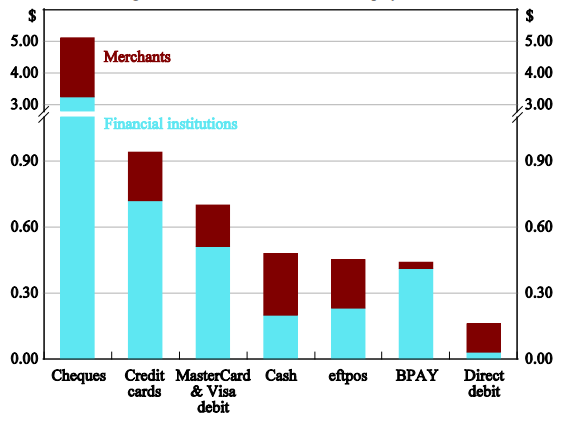
\includegraphics{figures/DirectResourceCosts.png}
\caption{Direct Resource Costs per average-sized transaction for each payment method\cite{RefWorks:271}}
\end{figure}

It should be obvious that moving from using cheques for transactions to using electronic transactions would be hugely beneficial to all parties in a transaction and that finanacial institutions would be doing everything possible to encourage transaction participants to move to electronic transactions over cheques and even cash. As financial institutions are able to pass the fees onto consumers, there is little incentive for them to switch to cheaper transaction mechanisms.

Overwhelmingly, however, Australians prefer non--cash transactions with only 18\% of the value of all transactions taking place in cash. Cash does, however, make up almost 50\% of the number of transctions indicating that most low value transactions take place using cash. This share may be expected to decrease with, as has previously been discussed, the likelihood that over 90\% of transactions will be conducted electronically by 2025\cite{RefWorks:262}.

\begin{figure}
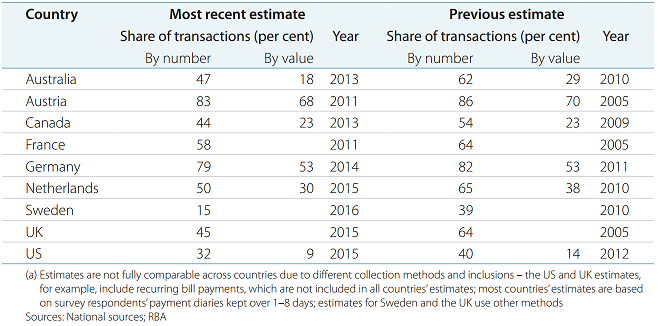
\includegraphics[scale=0.75]{figures/CashUseAcrossCountries.png}
\caption{Cash Use Across Countries\cite{RefWorks:270}}
\end{figure}


\subsection{Opportunity cost of electronic transactions to non-urban Australians}
Electronic transactions save a lot of time as well as money. It is obvious that if an Australian in a remote or regional setting has to travel several hours over rough roads to make a cash transaction that could be made electronically such as depositing cheques, salary or paying a mortgage or other bill, then it could literally cost them their lives in a car accident.  Taking aside the less risky nature of making a transaction electronically, if non--urban Australians need to travel more than walking distance to withdraw cash for their everyday needs in their local area is a non--trivial exercise. This is time that is better spent earning money than in travelling, even if the travel is only to the local post point to post a cheque. In fact, the time taken to complete an electronic transaction is substantially less than presenting a cheque. While using a credit or debit card takes less than half the time required to present a cheque for a transaction, using a contactless debit or credit card is almost twice as fast and is actually faster than using cash for a transaction. It can be seen that the rollout of contactless transaction systems such as Paypass, Paywave, Apple Pay et al, can shave time off the average person's transaction times over the course of a year and this translates into a difference in the opportunity costs for people depending on the transaction type.

It may seem unrealistic to say that making a transaction electronically will give a person back hours a week or put more money in their pocket at the end of the week but I present the anecdotal example of a lawyer who charges in `decimal time', that is they  bill their time to clients in six minute increments, as a model. This lawyer pays for a ticket to get a train to work each day and, by using paypass instead of cash they save enough time to catch the train that they would otherwise just miss. With another train not along for the next 15 minutes to an hour, saving a few seconds could earn them several hours of income each week that they would not otherwise be able to bill. Of course if the transaction was completely electronic, using a travel card such as Transport for NSW's Opal or Victorian Public Transport's myki that automatically tops up its stored value from the customer's credit card account, even more time would be saved and more money earned by this hypothetical lawyer.

Average opportunity costs, the lost earnings that were sacrificed for the time taken to make the transaction instead of earning salary,  have been measured for each transaction type and the differences are sobering.

\begin{quotation}
Combining the total time consumers use to make payments with estimates of the
value of this time suggest that the opportunity cost for consumers in making
payments is about \$2.6 billion per annum. Of this amount, per transaction, BPAY
and cheque payments are estimated to be the most expensive payment
instruments, at \$0.60 per transaction. At the other end of the spectrum, the
relative speed of contactless debit transactions impose a cost of \$0.13 per
transaction on consumers. Cash and credit card transactions are estimated to
cost \$0.18 and \$0.19 per transaction\cite[p5]{RefWorks:273}.
\end{quotation}



